%======================================================================
\NEWSEC
%======================================================================

\subsection{\ssState}

\begin{frame}[fragile,label=ss-state] 

\secframetitle{\ssState}

%  What is the current state of Enzo-P?  Well, it can do this.

%  This is a pure hydrodynamics problem run using Enzo-P with AMR
%  enabled, with somewhat non-physical initial conditions.

%  It uses an ``array of octrees'' AMR approach, which is simply a
%  uniform array of octrees.  Each Block in the hierarchy contains a
%  small grid of field variables, with size typically around 16^3 to
%  32^3.

%  Enzo-P is parallelized using Charm++ instead of MPI.  Charm++ is an
%  asynchronous data-driven parallel programming language extention to
%  C++.  Each block in the mesh hierarchy is a separate parallel task
%  in Charm, called called a ``chare''.  A key feature of Cello's AMR
%  Charm++ implementation is that it is fully distributed--there is
%  *no* hierarchy meta-data, which addresses a key limitation of
%  the current Enzo.

%  Enzo-P is also designed to be powerful yet easy to use.  While you
%  *can* implement test problem types in Enzo-P like you can Enzo, you
%  can also specify initial and boundary conditions directly in the
%  parameter file.  In this example, initial conditions were generated
%  using a PNG file as a logical mask---the density is initialized to
%  1.5 wherever the PNG file pixels are non-black, otherwise its set
%  to be 12 times less.  This approach means that common test problems
%  such as the implosion problem, Sedov blast wave, or double mach
%  reflection can be set up in the parameter file exclusively without
%  requiring any C++ coding.

\pause
\begin{center}
\begin{minipage}{4.5in}
\begin{minipage}{2.9in}
\only<2->{\vspace{-0.1in}\centerline{in 2014} \ \\ \vspace{-0.2in} \ANIMATEGRAPHICS{width=2.9in}{10}{Images/Daze/daze-0}{000}{100}}
\end{minipage} \ 
\begin{minipage}{1.45in}
\only<3->{\vspace{-0.1in}\centerline{in 2015} \ \\ \vspace{-0.2in}\ANIMATEGRAPHICS{width=1.45in}{10}{Images/1509/1509-0}{00}{56}}
\end{minipage}
\end{minipage}
\end{center}
\pause
\pause
\begin{minipage}[t]{1.2in}
\footnotesize
\vspace{0.1in}
\blockred
\begin{block}<+->{\textbf{Mesh refinement}}
\scriptsize
 \mbox{``array-of-octrees''} \\
 \mbox{field data on blocks} \\ \ \\
\end{block}
\end{minipage} \ \ 
\begin{minipage}[t]{1.0in}
\footnotesize
\vspace{0.1in}
\blockgreen
\begin{block}<+->{\textbf{Parallelism}}
\scriptsize
 Charm++\\
\mbox{blocks are ``chares''} \\
 \mbox{fully-distributed}
\end{block}
\end{minipage} \ \
\begin{minipage}[t]{1.6in}
\raggedright
\footnotesize
\vspace{0.1in}
\blockblue
\begin{block}<+->{\textbf{Parameters}}
\scriptsize
 \mbox{\code{Initial \{ density \{}} \\
 \mbox{\code{ value = [ 1.5, "daze.png",  }} \\
 \mbox{\code{\ \ \ \ \ \ \ \ \ \ \ 0.125 ]; \} \} }}
\end{block}
\end{minipage}

\end{frame}

%----------------------------------------------------------------------

\begin{frame}[fragile,label=ss-state] 
\secframetitle{\ssState}
\begin{center}
\begin{minipage}{4.5in}
\begin{minipage}{2.2in}
\only<2->{\centerline{in 2016}}
\end{minipage}
\begin{minipage}{2.2in}
\only<3->{\centerline{in 2017}}
\end{minipage}
 \vspace{0.2in} \\
\begin{minipage}{2.2in}
\begin{center}
\only<2->{\ANIMATEGRAPHICS{width=1.8in}{10}{trace-}{00}{99}}
\end{center}
\end{minipage} \
\begin{minipage}{2.2in}
\only<3->{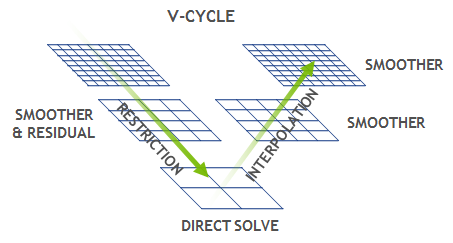
\includegraphics[width=2.0in]{hpgmg_v_cycle.png}}
\end{minipage}
\end{minipage}
\end{center}
\end{frame}

%----------------------------------------------------------------------

\begin{frame}[fragile,label=ss-state] 
\secframetitle{\ssState}
\begin{center}
\centerline{in 2018}  \ \\
\begin{minipage}{4.5in}
\begin{minipage}{2.2in}
\only<2->{\ANIMATEGRAPHICS{width=2.0in}{5}{Images/Cosmo/B3/dark-}{00}{21}}
\end{minipage} \
\begin{minipage}{2.2in}
\only<3->{\ANIMATEGRAPHICS{width=2.0in}{5}{Images/Cosmo/B3/mesh-}{00}{21}}
\end{minipage}
\end{minipage}
\end{center}
\end{frame}

